
\documentclass[../relatorio.tex]{subfiles}
\begin{document}
Durante a implementação, começou a tornar-se confuso gerir
o número crescente de classes.
Por esse motivo, decidiu organizar-se em \textit{Packages}.

A primeira versão da organização, consistiu, essencialmente,
em "transformar" o diagrama de componentes em pacotes.
Posteriormente, identificou-se um conjunto de contextos que permitiram uma melhor organização
das classes.

\begin{itemize}
    \item[SSClientes] {
          Corresponde ao sistema de gestão de clientes.\\
          Tratando-se de um sistema pequeno, não se efetuou nenhuma subdivisão.
          }
    \item[SSReparacoes] {
          Identificou-se três contextos de utilização:
          \begin{itemize}
              \item[Reparação]{
                    Toda a lógica relacionada com a Reparação, ReparaçãoProgramada e ReparaçãoExpresso.\\
                    Colocou-se, ainda, as classes de implementação utilizadas por si (CustoTotalReparacao e
                    ReparacoesPorMes).
                    }
              \item[Orcamento]{
                    Tal como o nome indica, corresponde às classes que implementam a lógica do Orçamento.
                    }
              \item[PlanoTrabalho] {
                    Sendo este um pacote comum aos dois anteriores, optou-se por colocar como um próprio,
                    passando os outros a utilizá-lo.
                    }
          \end{itemize}
          }
    \item[SSColaboradores] {
          Identificou-se, também, três contextos:
          \begin{itemize}
              \item[Colaboradores] {
                    Gestão dos colaboradores (adicionar ou alterar).
                    }
              \item[Balcao]{
                    Corresponde à interação do Funcionário de Balcão com os Equipamentos
                    (Receber ou Entregar).
                    Optou-se por colocar num pacote próprio para tornar as dependências menos
                    "aninhadas".\\
                    Eventualmente, poderia colocar-se esta lógica junto dos Colaboradores.
                    }
              \item[Agenda] {
                    Atendendo que tem uma implementação isolada, é fácil de perceber que
                    se encontra num contexto próprio e, portanto, foi-lhe atribuída um
                    pacote.
                    }
          \end{itemize}
          }
\end{itemize}

Ao utilizar a estrutura definida, ficou mais percetível o papel de cada classe.
Dizendo apenas o sistema em que se encontra, torna-se ineficiente e menos compreensivo,
pois pode não se conseguir atribuir, de imediato, uma classe a um contexto.

Será de referir que o diagrama de pacotes (\ref{img:diagrama_package}) desenvolvido se encontra
incompleto, por dúvida sobre a sua construção.

\begin{figure}[!ht]
    \centering
    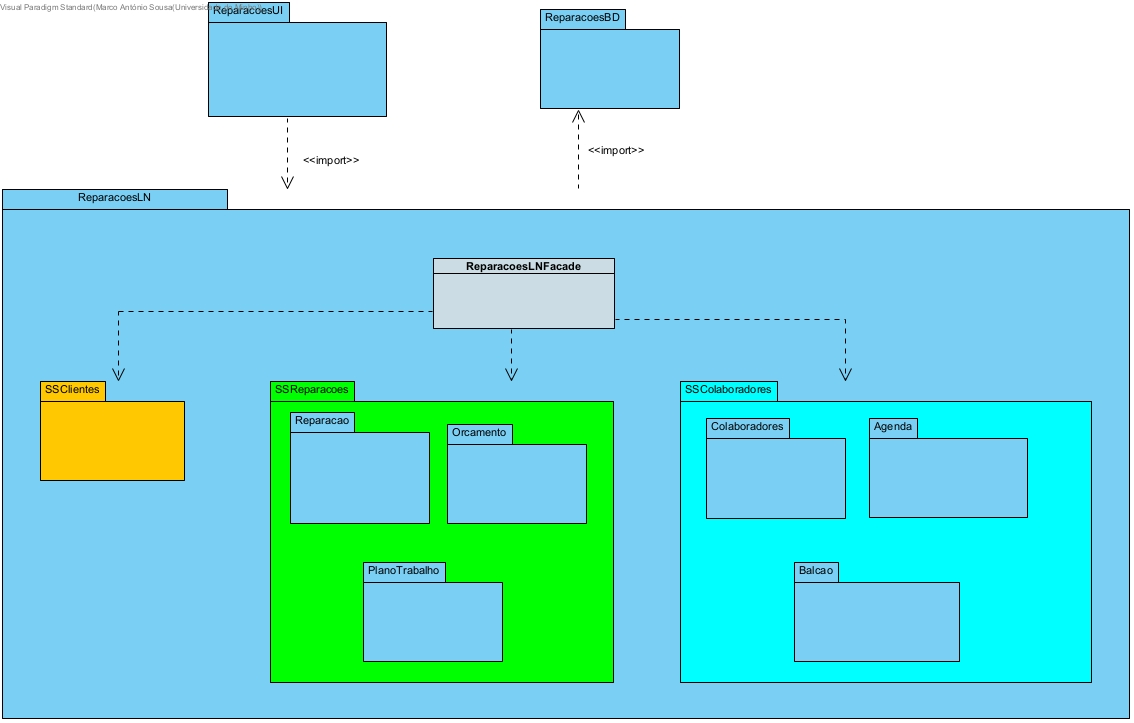
\includegraphics[width=\linewidth]{Reparacoes.jpg}
    \caption{Diagrama de Package} \label{img:diagrama_package}
\end{figure}
\end{document}